%%%%%%%%%%%%%%%%%%%%%%%%%%%%%%%%%%%%%%%%%%%%%%%%%%%%%%%%%%%%%%%%%%%%
\section{Overview (2 pages)}
\label{sec:fdsp-apa-intro}

\fixme{This is a first rough draft of the APA chapter. Some sections contain more information and detail than can be included in the TP, others contain just a list of content to be added. This draft, therefore, should not be read for detailed editing, but rather for overall layout and content. 2/25/2018}

%%%%%%%%%%%%%%%%%%%%%%%%%%%%%%%%%%%%%
%\subsection{Introduction}
%\label{sec:fdsp-apa-intro}

Anode Plane Assemblies (APAs) are the far detector elements utilized to sense ionization created by charged particles traversing the liquid argon volume inside the single-phase TPC.  The planes are interleaved with Cathode Plane Assemblies (CPAs) to establish the required electric fields and form drift volumes for the charged particles. Four 3.6~m wide drift regions are defined in each 10-kton DUNE far detector module, as shown in the end view in Figure~\ref{fig:FarDet-interior}, by two high voltage planes and three wire readout planes that run the 58~m length of the cryostat. 

Each Anode Plane Assembly is 6~m high and 2.3~m wide.  Figure~\ref{fig:FarDet-interior} also shows a schematic view of a partially assembled 10-kton TPC with vertically double hung anode plane frames (shown in red).  Twenty-five of these vertical stacks make up each span in the 58~m long detector.  Each 10-kton module, therefore, contains 150 APAs.

A single APA frame is covered by more than 3500 150~$\mu$m diameter Cu-Be sense wires laid in four planes: two angled induction planes (U and V), a vertically running collection plane (X), and an outermost grid layer (G) that is not read out but shields the first induction plane from charge as it approaches the grid in the argon volume.  The wires are wrapped around the frame from one side to the other, allowing all channels to be read out from one end only (the top or bottom) and minimizing the dead region between neighboring APAs. 
%such that there are 3 readout wire planes on each side, two induction planes (U and V) and an innermost collection plane (X).  There is also an outermost grid layer (G) that is not read out but shields the first induction plane from charge as it approaches the grid in the argon volume. 
Signals induced and collected on the wires are transferred through soldered connections to wire termination boards mounted at the end of the APA frame which in-turn connect directly to front-end readout electronics sitting in the argon. %Figure~\ref{APAschematic} shows a schematic of the wrapped wire planes, the shapes of signals created on the different planes, and the positioning of wire carrier boards mounted around the perimeter of the frame.  

The underlying support frames are made from stainless steel hollow tube sections that are precision machined and bolted together.  %XX wire carrier boards are screwed and epoxied to the perimeter of the frame that provide termination solder pads for wires and conductive traces to a front-end electronics pin connector. 
The frames are strung with wires using an automated wire placement and tensioning machine and soldered in place by hand.  A prototype winding machine has been designed and used to string full-scale APA frames at the Physical Sciences Laboratory (PSL) at the University of Wisconsin as well as at the Daresbury Laboratory in the UK for the ProtoDUNE project at CERN. This effort has greatly informed the design and production planning for the DUNE far detectors. %Figure~\ref{fig:APA-photos} shows the fabrication of the first ProtoDUNE APA module at PSL in Wisconsin in 2017.  

\begin{dunefigure}[Schematic view of a DUNE 10-kton TPC module]{fig:FarDet-interior}{Left: End-on schematic view of the active argon volume showing the four drift regions and anode-cathode plane ordering of the TPC inside the detector. Right: View of the partially installed DUNE TPC inside the membrane cryostat. The APAs are shown in red, CPAs are in cyan, field-cage modules in yellow/green.  Some of the field-cage modules are in their folded position against the cathode (providing aisle access during installation).}
\setlength{\fboxsep}{0pt}
\setlength{\fboxrule}{0.5pt}
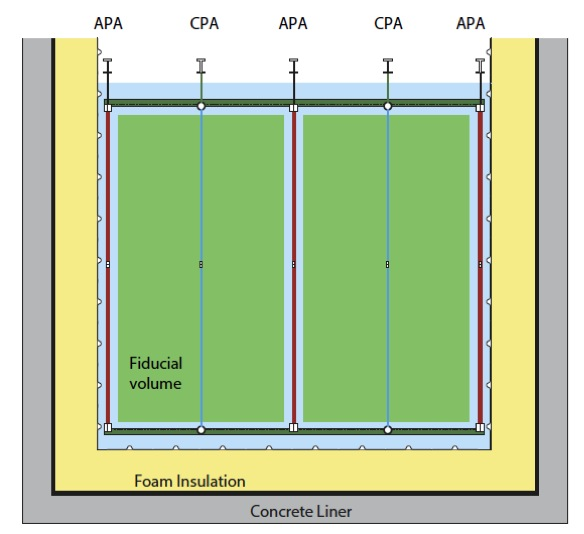
\includegraphics[width=0.41\textwidth, trim=0mm 3.7mm 0mm 0mm, clip]{FarDet-endview-SP.jpg}\hspace{0.05\textwidth}
\fbox{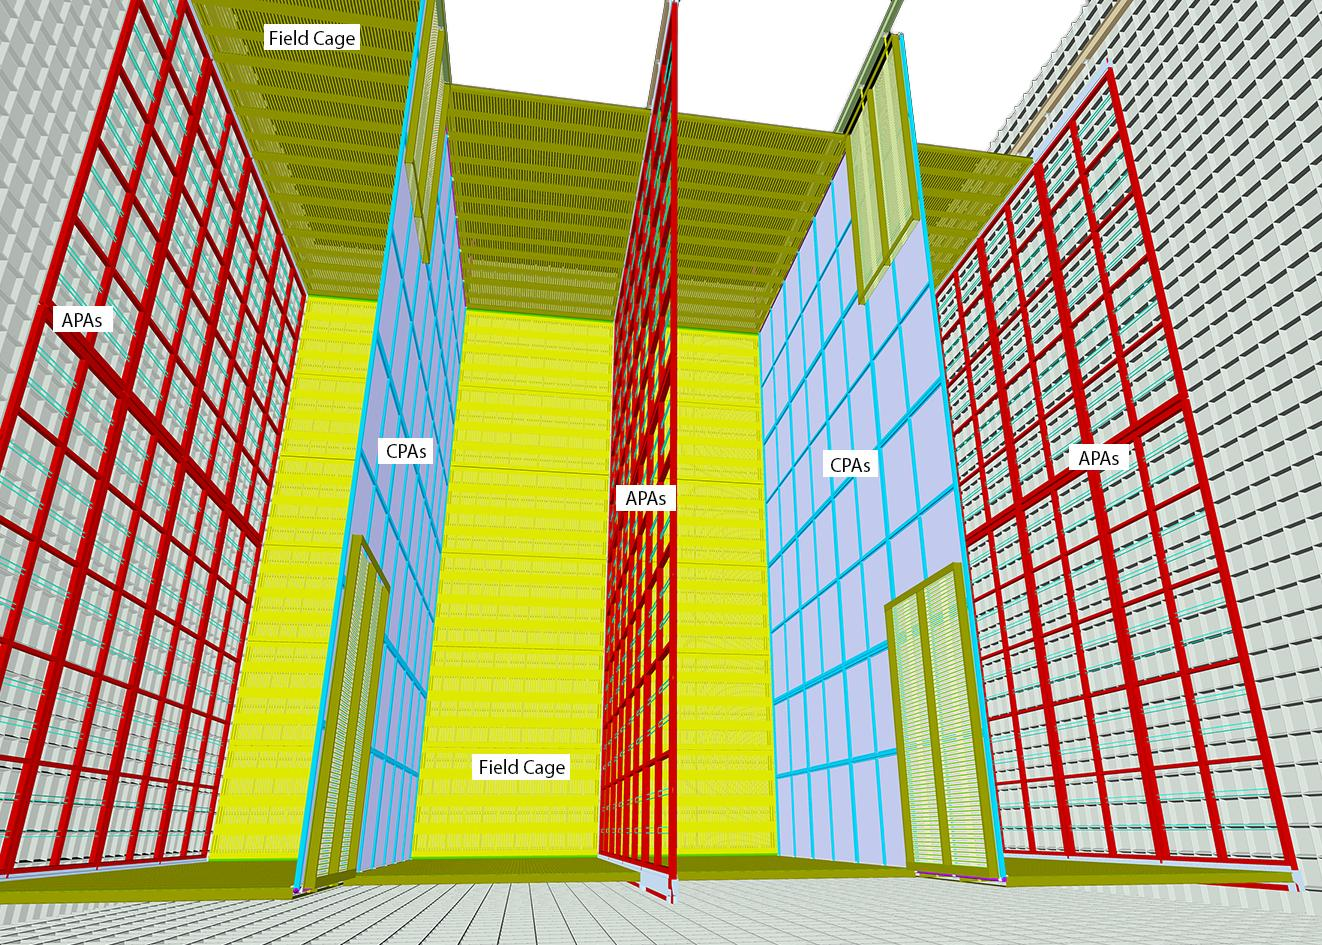
\includegraphics[width=0.5\textwidth]{tpc_floor_view.jpg}}
\end{dunefigure}

%\fixme{Include an image of the overall system, indicating its parts. Show how the system fits into the overall detector.}

%The operating principle is illustrated in Figure... (add figure)

%An APA consists of a rectangular framework with a fine wire mesh stretched across it, over which are wrapped four layers of sense and shielding wires......

%%%%%%%%%%%%%%%%%%%%%%%%%%%%%%%%%%%%%%%
\subsection{APA Design Requirements}
\label{sec:fdsp-apa-des-consid}


%%%%%  Design to identify MIPs -- wire pitch and other params
The APA design must enable identification of minimum-ionizing particles (MIPs). This is a function of several detector parameters, including: argon purity, drift distance, diffusion, wire pitch, and Equivalent Noise Charge (ENC).  DUNE-SP requires that MIPs originating anywhere inside the active volume of the detector be reconstructed with 100$\%$ efficiency.   The choice of wire pitch, of $\sim$5\,mm, for the wire layers on the APA, combined with key parameters for other TPC systems (described in their respective sections of the TDR), is expected to enable the 100$\%$ MIP identification efficiency.

%%%%% Locate vertices, determine fiducial vol, then back to vertex...?
DUNE-SP requires that it be possible to determine the fiducial volume (via analysis) to $<$1$\%$, which in turn requires reaching a vertex resolution of $\sim$1.5\,cm along each coordinate direction. (The fiducial volume, among other factors, determines the number of target nucleons, which is a component in estimating event rates.) The fine granularity of the APA wires enables excellent precision in identifying the location of any vertices in an event, (e.g., the primary vertex in a neutrino interaction or gamma conversion points in a $\pi^{0}$ decay), which has a direct impact on reconstruction efficiency.
In practice, the resolution on the drift-coordinate ($x$) of a vertex or hit will be better than that on its location in the $y-z$ plane, due to the combination of drift-velocity and electronics sampling-rate.  The physics performance requirements that drive the design of the APA are summarized in Table~\ref{tab:apaphysicsrequirements}.  %These are chosen to enable high-efficiency reconstruction throughout the entire active volume of the LArTPC.  

\begin{dunetable}[Physics requirements that motivate APA design parameters]{lr}{tab:apaphysicsrequirements}{Physics requirements that motivate APA design parameters.}   
Requirement & Value  \\ \toprowrule
MIP Identification & 100$\%$ efficiency \\ \colhline
High efficiency for charge reconstruction & $>$90$\%$ for $>$100 MeV \\ \colhline
Vertex Resolution (x,y,z) & (1.5 cm, 1.5 cm, 1.5 cm)\\ \colhline
\textbf{Particle Identification} & \\ 
Muon Momentum Resolution & $<$18$\%$ for non-contained \\
            & $<$5$\%$ for contained\\ 
Muon Angular Resolution & $<$1$^{\circ}$\\            
Stopping Hadrons Energy Resolution & 1-5$\%$\\
Hadron Angular Resolution & $<$10$^{\circ}$ \\ \colhline
\textbf{Shower identification} & \\
Electron efficiency & $>$90$\%$\\
Photon mis-identification & $<$1$\%$\\
Electron Angular Resolution & $<$1$^{\circ}$ \\
Electron Energy Scale Uncertainty & $<$5$\%$\\
\end{dunetable}

The size of the APAs is chosen for fabrication purposes, compatibility with over-the-road shipping, and for eventual transport to the 4850 level at SURF and installation into the membrane cryostat of a detector module. Sufficient shock absorption and clearances are taken into account at each stage.  The dimensions are also chosen such that an integral number of electronic readout channels and boards fill in the full area of the APA. The modularity of the APAs allows them to be built and tested at off-site production facilities, decoupling their manufacturing time from the construction of the membrane cryostat.

\fixme{Add ref to requirements document when it's ready, listing the most important ones in table 3.1.}  

%\fixme{By the end of the volume, for every requirement listed in this section, there should exist an explanation of how it will be satisfied.}

%%%%%%%%%%%%%%%%%%%%%%%%%%%%%%%%%%%
%\subsection{Scope}
%\label{sec:fdsp-apa-scope}

\begin{comment}
The scope of the Anode Plane Assembly (APA) system includes the continued procurement of materials for, and the fabrication, testing, delivery and installation of the following systems: 

\begin{itemize}
\item a framework of lightweight, rectangular stainless steel tubing;
\item a mesh layer attached directly to both sides of the APA frame;
\item layers of sense and shielding wires wrapped at varying angles relative to each other;
\item stacked head electronics boards, which are wire boards for anchoring the wires at the top (head) of the APA;
\item capacitive-resistive (CR) boards that link the wire boards to the cold electronics (CE);
\item side and foot boards along the other three edges of the APA with notches and pins to hold the wires in place;
%\item glue and solder;
\item modular boxes to hold the CE;
\item comb wire supports, mounted on cross braces distributed along the length of the APA, to prevent wire deflection; and
\item pin/slot pairs on the side edges of adjacent APAs to maintain coplanarity.
\end{itemize}
\end{comment}
